% !TeX root = ./kernel/easyExam.tex
\section*{Exercice 1 \MarksTwo}

\begin{enumerate}
      \item Décrivez brièvement le fonctionnement d'un réseaux intélligent.
      \item Donner la représentation de l’architecture d’un projet réseau intelligent.
            On insistera uniquement sur les couches principales de l'architecture.
      \item Citez en donnant les fonctions de chaque couches de l'architecture des réseaux intélligents.
      \item Citez 05 (cinq) protocoles des réseaux intélligents.
      \item Quelle est la couche de l'architecture des réseaux intélligents qui interagit directement avec les processus industriels ?
            Comment cette interaction se produit t-elle?
      \item Donnez la différence entre un réseaux dit "non intélligent" et un réseaux intélligent.
\end{enumerate}
La figure \ref{fig:iiot} montre le chef mécanicien vérifiant et contrôlant des robots robots d'automatisation des bras dans l'industrie intelligente d'usine sur le logiciel de système de surveillance en temps réel.

\begin{enumerate}
    \item Donnez trois (03) protocoles réseaux adaptés dans la mise en place de ce réseau intélligent industriel (voir figure \ref{fig:iiot}).
    \item Donnez les élements de chaque couche de l'architecture d'un réseau intélligent se trouvant sur la figure \ref{fig:iiot}.
    \item Donnez deux (02) avantages de ce réseau sur une industrie.
    \item Donnez deux (04) tâches à éffectuer afin d'éviter l'attaque des robots réseau sur les employés de cette l'industrie.
\end{enumerate}

\begin{figure}[!ht]
    \centering
    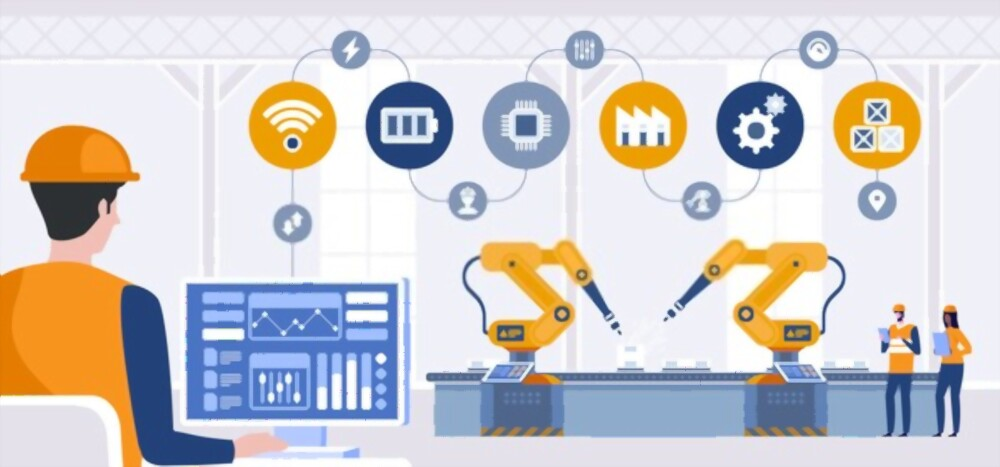
\includegraphics[scale=1.4]{../../figs/industrial_inttelings.jpg}
    \caption{Le chef mécanicien vérifie et contrôle des robots robots d'automatisation des bras dans l'industrie intelligente d'usine sur le logiciel de système de surveillance en temps réel.}
    \label{fig:iiot}
\end{figure}